\documentclass[11pt,leqno,oneside]{amsart}

\usepackage{../notes}
\newcommand{\Arg}{\operatorname{Arg}}
\newcommand{\Log}{\operatorname{Log}}
%%%%%%%%%%%%%% BEGIN CONTENT: %%%%%%%%%%%%%%

\title[Complex Analysis]{Complex Analysis}
\author{George H. Seelinger (inspired from class by David Sherman)}
\date{Fall 2016}
\begin{document}
\maketitle
\section{Lecture 1}
What makes complex analysis different than calculus and real analysis?

\begin{enumerate}
    \item Over the complex field, all polynomials factor completely.
    \item All the functions are infinitely differentiable and can thus be written as a power series.
    \item It is easier to describe important physics problems using complex analysis to solve partial differential equations.
    \item Some integrals can be solved using visual tricks and some integrals that are not solvable using calculus/real analysis omit solutions using complex analysis.

\end{enumerate}
\begin{example}
    The polynomial $x^2+10x+100$ cannot be factored in terms of real factors since its discriminant is negative. However, this can be factored over the complexes.
\end{example}
\begin{example}
    Describing physical phenemenon, such as the flow of a river over a log, is much easier using complex analysis.
\end{example}
\begin{example}
    Solving $\int_{-\infty}^{\infty} \frac{\cos 2x}{x^2+1} dx$ is almost impossible for a standard calculus student and in real analysis, one can show that the integral is finite, but solving it is difficult. In complex analysis, one can easily show that it is $\pi^2/e$.
\end{example}
\begin{example}
    $\int_{\gamma} \frac{\cos z}{z} dz = 2 \pi i $ times the number of counter clockwise rotations around $(0,0)$ in the complex plane.
\end{example}
\section{Lecture 2}
When doing complex analysis, it is important to develop a geometric intuition
for what is happening when you see functions of complex variables. The
following are some examples:
\begin{table}
    \centering
    \begin{tabular}{|c|c|}
        \hline
        $|z-w|$ & The distance from $z$ to $w$ \\
        $|z-1|=|z-i|$ & The locus of points equidistance from $1$ and $i$, ie a line. \\
        $|z-1|=3-|z-i|$ & The distance from $z$ to 1 and $z$ to $i$ add to 3, ie a parabola. \\
        $|z-1|=3+|z-i|$ & The upper part of a hyperbols (because the complex ordering). \\
        $|z-1|=2|z-i|$ & A circle (points that are twice as far from $1$ as from $i$). \\
        $|z-1|=\frac{2}{|z-i|}$ & An oval shape called a Cassini oval (product of distances is constant). \\
        \hline
    \end{tabular}
    \caption{Some real functions in complex form}
    \label{tab:func-descs}
\end{table}
Also note that $\ov{z}$ is $z$ reflected over the x-axis.

In $\R$, there are many ways to define $e^x$. One way is $e^x =
\sum_{n=0}^\infty \frac{x^n}{n!}$. Also, recall the taylor series expansions of
$\sin x$ and $\cos x$. We can define all these functions in complex $x$ using
the taylor series expansions.
\[
    e^{ix} = 1 + ix + \frac{(ix)^2}{2!} + \frac{(ix)^3}{3!} + \cdots = \cos x + i \sin x
\]
When $x$ is real, $|e^{ix}| = |\cos x + i \sin x| = \sqrt{\cos^2 x + \sin^2 x}
= 1$, so our rules in $\R$ still hold.

This formulation allows us to come up with the polar form of looking at complex
numbers. This boils down to $z = r e^{i \theta}$ where $r = |z|$ and $\theta
\in \arg z$. Note that $\arg z$ is the \emph{set} of (real) $\theta$ that solve
the equation. However, since $\arg$ is multi-valued, we say that $\Arg \in
\arg$ is the value that is between $(-\pi, \pi]$.

From this description, we get that $e^z e^w = e^{z+w}$ (follows from the power series). In particular, $(e^z)^n = e^{nz}, n \in \N$, This gives us \[
    \cos n \theta + i \sin n \theta = e^{in\theta} = (e^{i\theta})^n = (\cos \theta + i \sin \theta)^n
\]
This formula is often called \emph{DeMoivre's formula} and from it, we can
recover trig identities by expanding and equating the real and imaginary parts.

Overall, polar form is good for understanding multiplication and powers. For example, $\frac{1}{z} = \frac{1}{r} \exp{-i \theta}$.

We can also take roots effectively using polar form (look it up).

Finally, we can look at the stereographic projection (see textbook for picture) using the one-point compactification of $\C$, namely $\C^* = \C \cup \{\infty\} \cong S^2$.

We also get some nice correspondances from actions on the sphere as in the table. \\
    \begin{tabular}{|c|c|}
        \hline
        Equator & $|z| = 1$ \\
        Upper hemisphere & $\{|z| > 1\} \cup \{\infty\}$ \\
        Lines of lattitude & Circle centered at origin \\
        Lines of longitude & Rays from origin \\
        Circles on $S^2$ that do not contain the north pole & Circles on $\C^*$ \\
        Circles on $S^2$ that contain the north pole & Lines on $\C^*$ \\
        \hline
    \end{tabular}
\section{Lecture 3}

Let us continue to understand some basic functions in on $\C$. \\
\begin{tabular}{|c|c|}
    \hline
    $f(z) = iz$ & Rotation counter-clockwise by $\frac{\pi}{2}$. \\
    $f(z) = (1+i)z$ & Rotation counter-clockwise by $\frac{\pi}{4}$ and dilation by $\sqrt{2}$. \\
    $f(z) = z^2$ & Squares modulus and doubles the argument. \\
   \hline
\end{tabular} \\
Let us also examine $f(z) = z^{\frac{1}{2}} = \{w | w^2=z\}$. This is a multivalued function satisfying
\begin{align*}
    (|w|e^{i\theta})^2 = |z|e^{i \arg z} & \implies \begin{cases}
        |w|^2 = |z| \implies |w| = \sqrt{|z|} \\
        2\theta \in \arg z \implies \theta = \frac{\Arg z}{2}, \frac{\Arg z + 2\pi}{2}
    \end{cases} \\
    \ & \ \implies \ w = \sqrt{|z|}e^{\frac{\Arg z}{2}i}, \sqrt{|z|}e^{\frac{\Arg z + 2\pi}{2} i}
\end{align*}
\begin{defn}
    A branch of a multivalued function is a (continuous) choice of output on some domain.
\end{defn}
\begin{example}
    $z \mapsto \sqrt{|z|}e^{\frac{\Arg z}{2}i}$ is the principal branch of
    $z^{\frac{1}{2}}$ on $\C \smallsetminus (-\infty,0]$.
\end{example}

Now, let us consider $f(z) = e^z$. This is $f(z) = e^{x+iy} = e^x(\cos y +
i\sin y)$. Notice that $e^x$ is the modulus and $\cos y + i \sin y$ is the
argument. We also note that $e^z$ maps a grid of cartesian coordinates into a
grid of polar coordinates.

Next, consider the inverse of $e^z$, namely $\log z$ on $\C \smallsetminus
\{0\}$. We get that $\log z = w \implies e^w = z = e^{\Re w} \cdot e^{i \Im w}
= |z|e^{i \arg z}$. Thus we get that $\Re w = \ln|z|$ and $\Im w \in \arg z$.
When we take $\Im w = \Arg z$, we get $\Log z$. It is instructive to look at a
picture of $\Log z$'s graph.

From the above, we also note that $\cos z = \frac{e^{iz}+e^{-iz}}{2}$ and $\sin
z = \frac{e^{iz}-e^{-iz}}{2i}$. These identities are also useful for finding
$\cos^{-1}$ and $\sin^{-1}$. Also note that $\cosh z = \frac{e^z+e^{-z}}{2}$
and $\sinh z = \frac{e^z-e^{-z}}{2}$. In this sense, $\cosh$ and $\sinh$ are
rotations of $\cos$ and $\sin$ in the complex plane.

Coming back to the function $z^{\frac{1}{2}}$, it is important to discuss the
branch cut of the function. This creates a 1 dimensional complex manifold or
2 dimensional real manifold (plus some structure). A good treatement of this
will not be found here, but refer to any standard complex analysis textbook.

\section{Lecture 4}
When considering the stereographic projection representation of the complex
plane, consider that the following actions on the sphere have the following
effects in $z$.

\begin{tabular}{|c|c|}
    \hline
    Reflection over $xy$ & $f(z) = \frac{1}{\overline{z}}$ \\
    Reflection over $yz$ & $f(z) = -\overline{z}$ \\
    Reflection over $xz$ & $f(z) = \overline{z}$ \\
    Rotation by $\pi$ around $x$ & $f(z) = \frac{1}{z}$ \\
    Rotation by $\pi$ around $y$ & $f(z) = \frac{-1}{z}$ \\
    Rotation by $\pi$ around $z$ & $f(z) = -z$ \\
    \hline
\end{tabular}

To get a group out of these actions, one needs to add $f(z) = z$ and $f(z) =
\frac{-1}{\overline{z}}$. This forms a certain group of isometries on the
surface of a sphere ($\cong \Z_2 \times \Z_2 \times \Z_2$). This means that
these maps will map circles on a sphere to other circles on a sphere, which
also means that circles and lines on a complex plane will be mapped ot circles
and lines on a complex plane.

Actually note that the group $O(3)$ (of 3 by 3 matrices) is the group of all
isometries of the sphere. Geometrically, there are 4 types of isometries
\begin{enumerate}
    \item The identity
    \item Reflection over a plane
    \item Rotation around an axis
    \item A glide reflection (rotation then reflection over the equator).
\end{enumerate}
Note, just items 1 and 3 form the group $SO(3)$.

\begin{defn}
    Functions of $z$ that are orientation perserving are known as conformal
    maps and are also analytic. Similarly, functions of $\overline{z}$ are
    orientation flipping and are thus anti-conformal maps and are also
    anti-analytic.
\end{defn}

Treatment of phase factors is skipped because it is difficult to write up
without pictures.

\section*{Analysis Review}

\begin{defn}
A domain in $\C$ is convex if, for any two points in the domain, the line
between them is also contained in the domain.
\end{defn}
\begin{defn}
    A domain in $\C$ is star-shaped if there exists a point for which, when a
    line is drawn between it and any other point in the domain, the line is in
    the domain. Note that all convex domains are star-shaped, but not the other
    way around.
\end{defn}
\begin{defn}
    Let $f: \C \to \C$ be defined on a domain containing $z$. If $\lim_{\Delta
    z \to 0} \frac{f(z+\Delta z) - f(z)}{\Delta z}$ exists in $\C$, this number
    is called the \emph{derivative of $f$} at $z$ and we say that $f$ is
    differentiable at $z$.
\end{defn}

```Usual examples'' include $f(z) = z^n \implies f'(z) = nz^{n-1}$. Also note
that $f(z) = \overline{z}$ is not differentiable anywhere because the value of
the limit changes depending on if you approach in the real direction or the
imaginary direction.
\begin{defn}
    $f$ is \emph{analytic} on a domain if it is differentiable at all point on
    the domain and $f'(z)$ is continuous.
\end{defn}
We will see that the second assumption is superflous when we prove Goursat's
theorem later.

\begin{thm}
    Let $f(x+iy) = u(x,y)+iv(x,y)$ be defined on a domain. Then it is analytic
    if and only if $u,v$ satisfy the Cauchy-Riemann equations $u_x = v_y, u_y =
    v_x$ and these partials are continuous.
\end{thm}
\begin{proof}
    Assume $f$ is analytic. Then, take the limits of $\Delta z$ along the
    imaginary axis and the real axis and then equate. This should yield the
    Cauchy-Riemann equations.

    Conversely, take the Cauchy-Riemann equations and show that the limit
    exists using Cauchy-Riemann equations.
\end{proof}
\section{(9/6/2016) Lecture 5: Landau Notation and Cauchy-Riemann Equations}
\begin{rmk*}
    An aside at the beginning of lecture: recall $|z+i||z-i|=c$ from homework.
    It is true that any equation of the form $|p(z)| = c$ where $p$ is a
    complex polynomial and $c$ a nonnegative constant forms curves called ovals
    of Cassini. These are generally called polynomial lemniscetes. An open
    Erdos conjecture is as follows: \\

    All monic polynomials of degree $n$, the length of the polynomial
    lemniscete $|p(z)|=1$ is maximized by $z^n-1$.
\end{rmk*}

    A second aside about confusion concerning branch points and branch cuts.
    The general situation is that we have a multivalued function and we want to
    define a branch of it on some domain. Some things that could happen at 0:
    \\
    \begin{tabular}{|c|c|}
        \hline
        $\frac{1}{z}$ & Singly valued on $\C \smallsetminus \{0\}$, 0 is not a
        branch point. \\
        $z^{\frac{1}{2}}$ & Defined on 0, but 0 is a branch point. This yields
        a phase factor of $-1$. \\
        $\log z$ & 0 is a branch point, but there is no phase factor. \\ \ & Instead
        you add $2\pi i$ on a counter-clockwise loop. \\
        \hline
    \end{tabular}
    Recall that a branch point is a point where the one cannot define a
    continuous branch in a deleted neighborhood of the point. The minimum
    situation for all these listed functions with 0 as a branch point is that
    one can remove path from 0 to $-\infty$ from the domain.

    To emphasize further, ``the branch of $z^\frac{1}{2}$ on $\Re z > 1$ that
    is negative at 2'' is a valid sentence.

    \subsection*{Landau (``big oh'') notation}
    The idea behind Landau notation is that we want to bound one function in
    terms of another as the input $x$ goes to some $c$ (typically either 0 or
    $\infty$). This idea is used a lot in computer science and is an integral
    part of complexity analysis.

    \begin{defn}
        Say that $f$ is $O(g)$ if there is a positive $M$ in a neighborhood of
        $c$ where $|f(x)| \leq M|g(x)|$.
    \end{defn}
    Note, if there is a neighborhood where $g \neq 0$, this say that
    $\frac{|f(x)|}{|g(x)|}$ is bounded near $c$.
    \begin{defn}
        $f$ is $o(g)$ if $\forall \epsilon > 0$, there is a neighborhood of $c$
        where $|f(x)| < \epsilon |g(x)|$.
    \end{defn}
    Here, if there is a neighborhood where $g \neq 0$, this says that
    $\frac{|f(x)|}{|g(x)|} \to 0$.\\

    It is important to note that language here gets abused frequently.

    \begin{example}
        (At $\infty$), $f$ is $O(x^6)$, $g$ is $O(x^4)$. Then, $f+g$ is
        $O(x^6)$ and $fg$ is $O(x^10)$.
    \end{example}

    Some further consequences are that $f$ is bounded is the same as saying $f$
    is $O(1)$ and that saying $f$ goes to 0 is the same as saying $f$ is
    $o(1)$.

    \subsection*{Returning to differentiation}

    \begin{defn}
        A restatement of differentiability is that $f$ is differentiable at $x$
        if and only if $\exists c$ such that $f(x+\Delta x) = f(x) + c \Delta x
        + o(\Delta x)$ and if $f$ is differentiable, $c$ is the derivative of
        $f$ at $x$. Note that the $o(c)$ captures the essential notion of the
        derivative, since it essentially states that the error must go to zero
        and must be $o(\Delta x)$, ie, the error must approach zero faster than
        $\Delta x$.
    \end{defn}
    Note that the statement for complex differentiability is the same, but
    replace all $\Delta x$ by $\Delta z$ and replace $o(\Delta x)$ with $o(|
    \Delta z|)$. Now for an application: prove the Leibniz rule (product rule
    of differentiation) using landau notation.
    \begin{proof}
        \begin{align*}
            f(x+\Delta x)g(x+\Delta x) & = (f(x)+f'(x)\Delta x + o(\Delta
            x))(g(x)+g'(x) \Delta x + o(\Delta x)) \\
            \ & = f(x)g(x) + \Delta x(f'(x)g(x)+g'(x)f(x)) \\
            \ & \ + f'(x)f'(x)(\Delta
            x)^2 + f'(x)(\Delta x)o(\Delta x) + \dots \\
            & = f(x)g(x) + \Delta x(f'(x)g(x) + g'(x)f(x)) + o(\Delta x)
        \end{align*}
        Note the abusive notation, but it gets the desired result since the
        $o(\Delta x)$ terms go to 0 and thus the derivative is
        $f'(x)g(x)+g'(x)f(x)$.
    \end{proof}

    Now, recall that we had a theorem stating that a function is analytic if
    and only if it satisfies the Cauchy-Reimann equation.
    \begin{proof}
        Let us examine $f'(z) = \lim_{\Delta z \to 0} \frac{f(z+\Delta z) -
        f(z)}{\Delta z}$. Taking $\Delta z = \Delta x$ real, then $f'(z) =
        \lim_{\Delta x \to 0} \frac{u(x+\Delta x, y)+iv(x+\Delta x,y) -
        (u(x,y)+iv(x,y))}{\Delta x} = u_x(x,y)+iv_x(x,y)$.

        Similarly, taking $\Delta z = i \Delta y$, we get $f'(z) = \frac{u(x,
        y+ \Delta y) + iv(x+,y+\Delta y)}{i\Delta y} = -iu_y+v_y$. Thus,
        setting both parts equal, we get $v_x = -u_y$ and $u_x = v_y$.

        We will now prove the converse using Landau notation instead of limits.
        Now, we know that $f(z+\Delta z) =
        u(x + \Delta x, y + \Delta y) + iv(x+\Delta x, y + \Delta y)$. We will
        choose to work with the real part first.
        \begin{align*}
            u(x+\Delta x, y + \Delta y)  & = u(x, y+ \Delta y) + \Delta x
            u_x(x,y+\Delta y) + o(\Delta x) \\
            \ & \text{ using the }x\text{ derivative.} \\
            \ & = u(x,y) + \Delta y u_y(x,y) + o(\Delta y) + \Delta x
            u_x(x,y+\Delta y) + o(\Delta x) \\
            \ & \text{ using the }y\text{ derivative.} \\
            \ & = u(x,y) + \Delta y u_y(x,y) + o(\Delta y) + \Delta x
            (u_x(x,y)+o(1)) + o(\Delta x) \\
            \ & \text{ using the continuity of }u_x\\
            \ & = u + \Delta y u_y + \Delta x u_x + o(\Delta y) + o(1)\Delta x
            + o(\Delta x) \\
            \ & = u + \Delta y u_y + \Delta x u_x + o(|\Delta z|)
        \end{align*}
        Similarly, we can do this to get $iv(x+\Delta x, y + \Delta y) =
        i(v+\Delta y v_y + \Delta x v_x + o(|\Delta z|))$. So now, continuing
        with $f$ and applying the Cauchy-Riemann equations, we get
        \begin{align*}
            f(z+\Delta z) & = u + iv + \Delta y (-v_x) + \Delta x u_x + i\Delta
            y u_x + i \Delta x v_x + o(|\Delta z|) \\
            \ & = u + iv + \Delta z(u_x+iv_x)+o(|\Delta z|)
        \end{align*}
        So, $f'(z) = u_x+iv_x$, which we assumed continuous, so $f$ is analytic.
    \end{proof}
    \section{(9/8/2016) Lecture 6: Developing Intuition for Complex Differentiation}
    In class, we first completed an exercise imagining the graph of $2i$
    raised to various powers. The end result was that these graphs always
    produce (possibly degenerate) spirals. Two graphs are provided here,
    but once raised to a complex power, the graphs produce spirals that
    increase their modulus exponentially, and so, at scale, the graph is rather
    unenlightening.

    \begin{figure}[h]
        \centering
        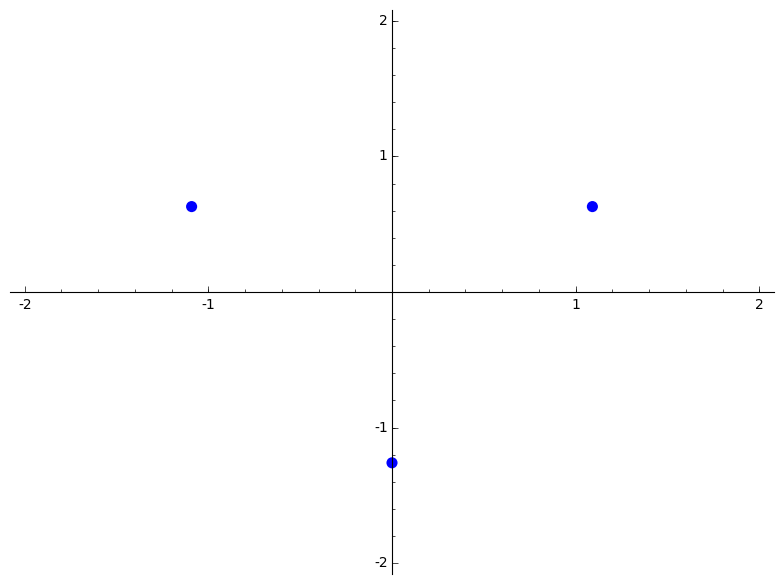
\includegraphics[scale=0.2]{images/2i-to-one-third.png}
        \caption{$2i^{\frac{1}{3}}$}
        \label{fig:2i13}
    \end{figure}
    \begin{figure}[h]
        \centering
        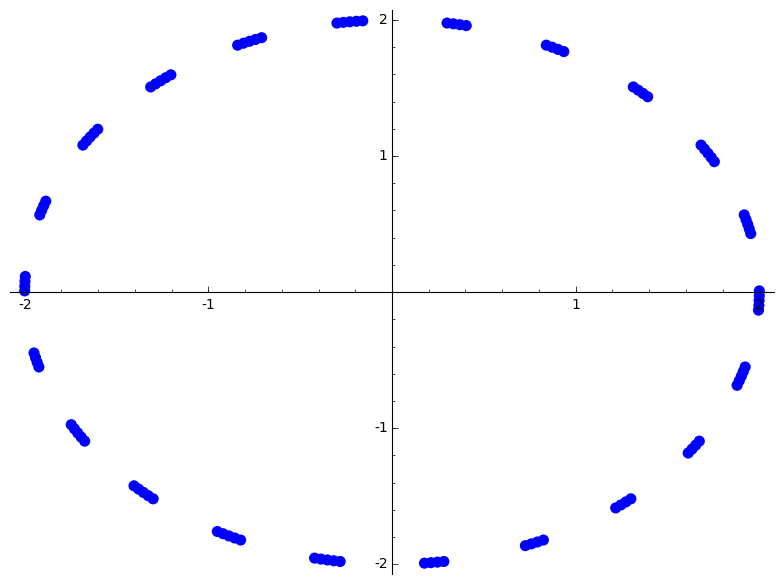
\includegraphics[scale=0.2]{images/2i-to-1-over-pi.png}
        \caption{$2i^{\frac{1}{\pi}}$ first $k = 0,1, \ldots, 100$}
        \label{fig:2i1pi}
    \end{figure}

    Now, a general definition of differentiability for $\R^n$ spaces is as
    follows.
    \begin{defn}
        A function $f: \R^m \to \R^n$ is differentiable at $x$ if $f(x+h) =
        f(x)+D(h)+o(h)$ where $D: \R^m \to \R^n$ is linear (a matrix). In fact,
        $D$ is the Jacobian matrix of partial derivatives and $f(x)+D(h)$ is
        the tangent plane.
    \end{defn}
    For a complex function $f: \C \to \C$, we write $f = u+iv$ where $u,v: \R^2
    \to \R$. When $u,v \in C^1$, $D = \left( \begin{array}{cc}
        u_x & u_y \\
        v_x & v_y
    \end{array}\right)$. As a reminder, complex differentiability happens when
    we have real differentiability plus the function satisfied the
    Cauchy-Riemann equations. Then, note that $\det D = u_x^2 + v_x^2 =
    |u_x+iv_x|^2 = |f'(z)|^2$. Thus a function $z+h \mapsto f(z) + f'(z)h$
    dilates $h$ by $|f'(z)|$ and rotates it by $\arg f'(z)$. The consequence of
    this is that analytic maps take squares in the input to squares in the
    output and they are orientation preserving. Thus, we get the following
    \begin{rmk}
        If $f$ is analytic on $D$, $z \in D, f'(z) = 0$, then there is a
        neighborhood $U$ with $z \in U \subset D$ on which $f$ is one-to-one
        with analytic inverse satisfying $f^{-1}(f(z))' = \frac{1}{f'(z)}$.
        This is the inverse function theorem and it applies since the Jacobian
        is invertible.
    \end{rmk}
    A natural question to then ask is how are branches affected by
    differentiation. Let us show a few examples.
    \begin{example}
        \begin{enumerate}
            \item $\frac{d}{dz}(\log z) = \frac{1}{z}$ where we are using any
                branch of $\log$. $z = e^{\log z} \implies 1 = e^{\log z} \cdot
                (\log z)' \implies \frac{1}{z} = (\log z)'$. Thus, the choice
                of branch for $\log$ does not affect the derivative in this
                case.
            \item $\frac{d}{dz}(z^{\frac{1}{2}})$ depends on the branch. $z =
                (z^{\frac{1}{2}})^2 \implies 1 =
                2(z^{\frac{1}{2}}(z^{\frac{1}{2}})'$ which gives us
                $(z^{\frac{1}{2}})' = \frac{1}{2(z^\frac{1}{2})}$. Thus, the
                $z^\frac{1}{2}$ in the final result is the same branch as the
                branch that was differentiated.
        \end{enumerate}
    \end{example}

    \begin{defn}
        A function $u: \R^n \to \R$ is \emph{harmonic} if it is a $C^2$
        solution to $\Delta u = 0$. Note that $\nabla^2u = \Delta u$ and is
        called the Laplacian.
    \end{defn}
    Harmonic functions will turn out to be $C^\infty$, but we cannot prove this
    yet. Note also that if $f = u+iv$ is analytic, then $u$ is harmonic. This
    follows because $u_{xx}+u_{yy} = u_{xx}+(-v_x)_y = u_{xx}-v_{yx} =
    u_{xx}-u_{xx} = 0$. There is an almost converse which states that ``a
    harmonic function is locally the real part of an analytic function.'' That
    is, on a neighborhood of any point, there is a $v$ with $u+iv$ analytic locally.
    Such a $v$ is called a \emph{harmonic conjugate} (unique up to an additive
    constant), e.g., there is an $x$ such that $u=xy$ satisfying \[
        \begin{cases}
 u_x = v_y = y \\
 u_y = -v_x = x. \\
    \end{cases}
\]
This is a PDE satisfied by the solution $\frac{y^2-x^2}{2} + C$. So, we get
that $xy+i\left( \frac{y^2-x^2}{2} \right)$ is analytic. In terms of $z$, this
conjugate is $f(x) = \frac{-iz^2}{2}$. Also note that the local part of the
definition is necessary. For instance $\frac{1}{2} \log(x^2+y^2)$ is harmonic
on $\R^2 \smallsetminus \{(0,0)\}$. \\

Some follow up facts to note are
\begin{itemize}
    \item All harmonic functions of $\R$ have the form $ax+b$.
    \item $u+v$ is harmonic.
    \item $uv$ is not harmonic.
    \item $u_x$ is harmonic.
    \item If $v$ is a harmonic conjugate of $u$, the harmonic conjugate of $v$
       is $-u$. Thus, note that harmonic conjugation is not an unordered pair.
    \item $u+iv$ is analytic implies that $v-iu$ is analytic.
\end{itemize}
\subsection*{Conformal Maps}
\begin{defn}
    If $f$ is analytic in a neighborhood at $z_0$ and $f'(z_0) \neq 0$, then
    $f$ is \emph{conformal} at $z_0$. This is the same as saying directed
    angles are preserved by $f$ at $z_0$.
\end{defn}
\begin{defn}
    A \emph{conformal mapping} between domains is a one-to-one $C^1$ function
    that is conformal at each point.
\end{defn}
Note the following implications.
\begin{itemize}
    \item $f: D \to V$ that is one-to-one and analytic is conformal.
    \item If $f$ is analytic at $z_0$ and $f'(z_0) \neq 0$, then $f$ maps a
        neighborhood of $z_0$ conformally onto the image.
\end{itemize}

\section{(9/13/2016) Lecture 7}
In general, a real differentiable function from $\R^2 \to \R^2$ will map some
small square to some small parallelogram modulo a small
perturbation. Furthermore, the ratio of the areas is the determinant of the
Jacobian. Now, if $f: \C \to \C$ is analytic and if $f'(z) \neq 0$, the map will
map a small square to another square modulo a small amount of error. This is an
essential difference between these types of functions. Thus, analytic maps are
conformal where $f' \neq 0$. \\

What if $f' = 0$?
\begin{example}
  Take $f(z) = z^2$ at 0. Then, $f(z)$ doubles angles, and is thus not angle
  preserving and thus not conformal at 0.
\end{example}

\begin{defn}
  A \emph{conformal equivalence} between domains is a one to one onto
  conformal/analytic map between them.
\end{defn}
\begin{example}
  $\{-\frac{\pi}{2} < \Im z < \frac{\pi}{2}\}$ is conformall equivalent to
  $\{\Re z > 0\}$ using the map $f(z) = e^z$.
\end{example}

A general question in complex analysis is ``given two domains, find a conformal
equivalence if one exists.''

Since conformal maps preserve angles, it is key to note they preserve
orthogonality.

\begin{rmk}
  Harmonic functions are exactly the functions that are locally the real parts
  of analytic functions. That is, given $u$, there exists on a neighborhood of
  any point and a $v$ defined on that neighborhood such that $u+iv$ is
  analytic.
\end{rmk}

\begin{example}
  \textbf{Non-example}: $\ln r$ on $\R^2 \textbackslash \{(0,0)\}$. There is no
  harmonic conjugate that works for the entire domain. A harmonic conjugate
  would be a branch of $\arg$, so $z \mapsto \ln|z|+i\arg z$ would have to be
  analytic. However, that is not possible since no branch of $\arg$ can be
  continuous for the entire domain.
\end{example}

\subsection{Linear Fractional Transformations}
\begin{defn}
    A \emph{linear transformation} is of the form $az + b$ with $a,b \in \C$.
\end{defn}
\begin{defn}
    An \emph{affine transformation} is a nonzero linear transformation.
\end{defn}
\begin{defn}
    A \emph{linear fractional transformation} is a map of the form $z \mapsto
    \frac{az+b}{cz+d}$ with $a,b,c,d \in \C$ and $ad-bc \neq 0$. These are also
    called fractional linear transformations and M{\"o}bius transformations.
  \end{defn}

  Some facts about LFTs:
  \begin{itemize}
  \item LFTs are unchanged if $a,b,c,d$ all multiplied by $\lambda \neq 0$.
  \item LFTs are defined at $\infty$.
  \item LFTs are one-to-one, onto maps from $\hat{\C} \to \hat{\C}$ with
    derivative non-zero. Thus, they are exactly the conformal equivalences from
    $\hat{\C} \to \hat{\C}$.
  \item LFTs are closed under inverse and composition. Thus, they have a group
    structure. A good treatment of this is in Gamelin in section II.7.
  \item Given distinct $z_1,z_2,z_3$ and distinct $w_1,w_2,w_3$, these exists a
    unique LFT taking $z_i$ to $w_i$.
    \item An LFT is a composition of linear maps and the inversion
      $\frac{1}{z}$. So, an LFT takes circles in $\hat{\C}$ to circles in
      $\hat{\C}$.
  \end{itemize}

  \subsection{Line Integrals}
  Line integrals are integrals of the form $\int_\gamma Pdx + Qdy$ where
  $\gamma$ is a path. To solve these, one usually parametrizes the path or uses
  theorems such as Green's theorem.
  \begin{defn}
    We call the integrand \emph{closed} if $P_y = Q_x$. We call the integrand
    \emph{exact} if there exists an $h(x,y)$ such that $h_x = P, h_y = Q$. Thus,
    if we have $h_xdx+h_ydy$, we would say this is an ``exact differential with
    $h$ as a primitive.''
  \end{defn}
  Note that if a vector field is exact, that is the same as saying it is
  independent of path or that integrals over loops are 0.
  \begin{rmk}
    \begin{itemize}
    \item If a differential is exact, then it is closed.
    \item If a differential is closed on a star-shaped domain, it is exact
    \end{itemize}
  \end{rmk}
  \begin{example}
    $\frac{-ydx+xdy}{x^2+y^2} = \Im \frac{1}{z}dz$ on $\R^2 \textbackslash
    \{(0,0)\}$ is closed but not exact.
  \end{example}
  Finally, to make notions of path precise, we have the following.
\begin{defn}
    A \emph{path} is a continuous parametrized function $f:[a,b] \to \C$.  A
    path is \emph{simple} if it is injective (ignoring the endpoint).  A path is
    \emph{closed} if $f(a) = f(b)$.  The \emph{trace} of a path is its image
    $f([a,b])$.  A path is \emph{smooth} if $f(t)$ can be expressed as $(x(t),
    y(t))$ for $x$ and $y$ smooth (such a path is also called a \emph{curve}).
    A \emph{piecewise} path is a concatenation of paths (two paths must share an
    endpoint to be concatenated).
  \end{defn}

  Finally, we conclude with the following
  \begin{thm}
    A harmonic function on a star shaped domain has a harmonic conjugate.
  \end{thm}
  \begin{proof}
    Suppose $u$ is harmonic, then $-u_ydx+u_xdy$ is closed. So, it is also
    exact. Let $v$ be a primitive. Then $v_x = -u_y, v_y=u_x$. Thus, $u+iv$ is
    analytic. (Check this proof.)
  \end{proof}
  \section{(9/15/2016) Lecture 8}
  Integrals of closed forms $\{Pdx+Qdy, Q_x = P_y\}$ are invariant
  when
  \begin{itemize}
  \item the path is deformed, fixing endpoints.
  \item a loop is deformed.
  \end{itemize}

  A physical application would be with fluid flow. The example
  provided in class is a the top half of a log lying at the bottom of
  a riverbed. We can create a conformal equivalence with $f(z) =
  z+\frac{1}{z}$ between the flow lines of this river and the flow
  lines of a river with no log.

  \begin{defn}
    A function on $\R^2$ (or $\R^n$) has the \emph{mean-value
      property} (MVP) on a domain if its value at any point is the
    average of its values on any sufficiently small circle (or sphere)
    centered at the point. In other words, $u(z_0) = \frac{1}{2\pi}
    \int_0^{2\pi} u(z_0+re^{i\theta}) d\theta$.
  \end{defn}
  An amazing consequence of this definition is that it is the same
  thing as being harmonic. In Gamelin, there is a treatment about how
  harmonic on $\R^2$ implies MVP. The idea is that $\frac{d}{dr}$(
  average on circle of radius $r$) $=0$. Then, the average is
  continuous as $r \to 0$, so the averages must all be $u(z_0)$. \\

  Note that, in $\R$, MVP implies harmonic (linear).

  \subsection*{Maximum Principles}

  \begin{thm}[``Strict Maximum Principle'' for real harmonic functions]
    If $u$ is a harmonic, real-valued function and $u \leq M$ on a
    domain and $u(z_0) = M$ for some $z_0$, then $u \equiv M$. This is
    the same as saying ``no peaks or pits.''
  \end{thm}
  \begin{proof}
    By MVP, $u(z_0)$ is the average of its values at a sufficiently
    small circle centered at $z_0$, but these values are all $\leq M$,
    so they must all be $M$. So, $u \equiv M$ on a small disk centered
    at $z_0$. So $\{u = m\}$ is open. It is also open by continuity of
    $u$. A non-empty clopen subset of a domain is the whole domain, so
    $u \equiv M$. 
  \end{proof}

  \begin{thm}[Strict maximum principle for complex harmonic functions]
    Same as above principle, except $|f(z)| \leq M$ and $|f(z_0)| =
    M$. 
  \end{thm}
  \begin{proof}
    We may assume $M \neq 0$. Then $|f(z_0)| = M \implies f(z_0) =
    Me^{i\theta}$. Consider the same hypothesis holds for
    $e^{-i\theta}f$, so $u = \Re e^{-i\theta}f$. Then, $u \leq M$ and
    $u(z_0) = M$. So by previous theorem, $u \equiv M$, $M \geq
    |e^{-i\theta}f| \geq u \equiv M$. This tells us that
    $e^{-i\theta}f \equiv M \implies f = Me^{i\theta}$.
  \end{proof}
  \begin{thm}[``Maximum modulus principle'']
    If $f$ is complex harmonic on a bounded domain and extends
    continuously to the boundary, then $f$ attains its maximum modulus
    on the boundary. 
  \end{thm}
  \begin{proof}
    $|f|$ is continuous on compact $D$, so the maximum is attained
    somwhere ?? in 0, so $f$ is constant by previous theorem. CHECK THIS!
  \end{proof}
  \section{(9/20/2016) Lecture 9: Complex Line Integrals}
  A complex line integral is an integral of the form $\int_\gamma
  f(z)dz$ where $\gamma$ is some path in the complex plane, $f(z)$ is
  some complex valued function, and $dz = dx + idy$. Just like a real
  integral, it can be phrased as $\lim \sum_{i=1}^n
  f(z_i^*)(z_{i+1}-z_i)$ and can be evaluated by parametrizing the
  path and function. \\

  We can also provide an upper bound on such integrals by noting the
  following:
  \begin{align*}
    |\int_\gamma f(z)dz | & \cong |\sum f(z)(z_{i+1}-z_i)| \\
    \ & \leq \sum |f(z_i^*)||s_{i+1}-z_i| \\
    \ & \leq \max_\gamma |f(z)| \sum |z_{i+1}-z_i| \\
    \ & \cong \max_\gamma |f(z)| \cdot \int_\gamma ds \\
    \ & (\max |f(z)|)(\operatorname{length} \gamma)
  \end{align*}
  This is called the ML estimate.

  \begin{example}
    Consider $\oint_{|z|=R} z^n dz$. We can parametrize this with
    $z(t) = Re^{it}, t \in (0,2\pi]$. Then, $z'(t) = iRe^{it}$ and we
    get our integral to be $\int_0^{2\pi} (Re^{it})^n iRe^{it} dt =
    R^{n+1} i \int_0^{2\pi} e^{it(n+1)} dt =
    \begin{cases}
      0 & \text{ if } n \neq -1 \\
      2 \pi i & \text{ if } n=-1
    \end{cases}.$
  \end{example}
  However, just like in calculus, we can also evaluate integrals using
  primitives or anti-derivatives. A primitive for $f$ is an analytic
  $F$ with $F'=f$.
  \begin{thm}[Fundamental Theorem of Calculus (Complex Version)]
    $\int_\gamma F'(z)dz = F(\text{end}) - F(\text{start})$
  \end{thm}
  This statement is exactly the same as the standard version.
  \begin{example}
    Consider $\oint_{|z|=R} z^n dz$. If $n \neq 1$, then $z^n$ has
    primitive $\frac{z^{n+1}}{n+1}$ on $\C \textbackslash
    \{0\}$. However, if $n=-1$, primitives of $\frac{1}{z}$ are
    branches of $\log z$ and thus cannot be continuously defined on
    $|z|=R$. 
  \end{example}
  In notes, there is a proof, but I am not sure why it is there...
  \begin{thm}
    If $f$ is analytic on a star-shaped (simply connected) domain,
    then it has a primitive.
  \end{thm}
  \begin{proof}
    Let $f=u_iv$. Consider $udz-vdy$. This differential is closed
    because $u_x = v_y$ by the Cauchy-Riemann equations. Now, since it
    is closed on a star-shaped domain, it is exact. So, there exists a
    $U$ with $U_x = u$ and $U_y = -v$ by definition of exact. Now,
    also note that $U$ is harmonic because $\Delta U = U_{xx} + U_{yy}
    = u_x-v_y = 0$ where the last equality follows from the
    Cauchy-Riemann equations. So, $U$ has a harmonic conjugate $V$
    since it is on a star-shaped domain. Thus, we have $F = U+iV$ that
    is analytic and note that $F' = U_x + iV_x = U_x-iU_y = u+iv = f$. 
  \end{proof}
  Note that in this situation, we have $F(z) = \int_{z_0 \to z}
  f(z)dz$ is well-defined where $z_0 \to z$ is any path from $z_0$ to
  $z$.
  \section{(9/22/2016) Lecture 10: Integral Formulas}
  Continuing from above, we ask what happens if the domain is not
  simply connected eith $f = u+iv$ where $u,v \in C^1$? We have that
  $f(z)dz$ is closed, which gives us $(u+iv)(dx+idy) =
  (u+iv)dx+(-v+iu)dy$. Next, we have $u_y+iv_y = -v_x+iu_x$, giving us
  the Cauchy-Riemann equations. Thus $f$ is analytic.
  \begin{thm}[Cauchy Integral Theorem]
    If $f$ is analytic on a bounded domain with piecewise smooth
    boundary and $f$ extends continuously to the boundary, then
    $\int_{\partial D} f(z)dz = 0$
  \end{thm}
  \begin{proof}
    By Green's Theorem
  \end{proof}
  Note that $\partial D$ is oriented with domain on the left. So, on
  an annulus, the boundary is counter clockwise on the outer boundary
  and clockwise on the inner boundary.
  \begin{example}
    Does $\frac{1}{z}$ of $\frac{1}{z^2}$ have an anti-derivative on
    punctured plane or slit plane? \\

    Both have an anti-derivative on the slit plane because the slit
    plane is star-shaped. On the punctured plane, $\frac{1}{z^2}$
    clearly has anti-derivative $\frac{-1}{z}$, but $\frac{1}{z}$ does
    not because $\oint_{|z|=1} \frac{1}{z}dz \neq 0$. 
  \end{example}

  \begin{thm}[Cauchy Integral Formula]
    Let $f$ be analytic on a bounded domain $D$ with piecewise smooth
    boundary where $f$ extends continuously to the boundary. Then, for
    any point $z \in D$, we have $\frac{1}{2\pi i} \int_{\partial D}
    \frac{f(w)}{w-z}dw = f(z)$. 
  \end{thm}
  The amazing thing about this formula is that the values of $f$ on
  the boundary completely determine $f$ on the interior. Such a
  property does not exist for real functions in general.
  \begin{proof}
    Find $\epsilon > 0$ small enough so $D_\epsilon(z) \subset D$. By
    the Cauchy Integral Formula,
    \[0 = \int_{D \textbackslash \overline{D_\epsilon(z)}}
      \frac{f(w)}{w-z}dw = \int_D \frac{f(w)}{w-z}dw -
      \int_{C_\epsilon} \frac{f(w)}{w-z}dw.\]
    So, it suffices to show $\frac{1}{2 \pi i}\int_{C_\epsilon}
    \frac{f(w)}{w-z}dw = f(z)$. So, let us parametrize $w(\theta) =
    z+\epsilon e^{i\theta}, \theta \in [0,2 \pi)$. Then, we get that
    $\frac{1}{2 \pi i}\int_{C_\epsilon} \frac{f(w)}{w-z}dw =
    \frac{1}{2\pi i}\int_0^{2 \pi} \frac{f(z+\epsilon
      e^{i\theta}}{\epsilon e^{i\theta}} i \epsilon e^{i \theta}
    d\theta = \frac{1}{2\pi}\int_0^{2 \pi} f(z+\epsilon e^{i \theta})
    d \theta = f(z)$ by the mean value property. 
  \end{proof}
  Note that we could have also proceeded by saying, for small
  $\epsilon$, we have that $f(z+\epsilon e^{i \theta}) \cong f(z)$ by
  continuity, so the integral divided by $2 \pi$ is arbitrarily close
  to $f(z)$.

  \begin{thm}[Generalized Cauchy Integral Formula]
    Same hypotheses as the Cauchy Integral Formula, but let $m \in
    \N$. Then, $f^{(m)}(z) = \frac{m!}{2 \pi i} \int_{\partial D} \frac{f(w)}{(w-z)^{m+1}}dw$
  \end{thm}
  \begin{cor}
    Analytic functions are $C^{\infty}$ and harmonic functions are $C^{\infty}$.
  \end{cor}
  \begin{proof}[``Proof'']
    $u$ harmonic implies there exists a harmonic conjugate $v$ on a
    neighborhood. Thus, $u+iv$ is analytic, so it is $C^{\infty}$ and
    thus $u$ is $C^{\infty}$. 
  \end{proof}
  \begin{proof}[Proof of Generalized Cauchy Integral Theorem]
    (case $m=1$): We have $\frac{f(z+\Delta z)-f(z)}{\Delta z} =
    \frac{1}{2 \pi i \Delta z} \int_{\partial D} \left[
      \frac{f(w)}{w-(z+\Delta z)} - \frac{f(w)}{w-z} \right]
    dz$. Multiplying to get a common denominator, we get that this is
    $\frac{1}{2 \pi i \Delta z}\int_{\partial
      D}\frac{f(w)(w-z)-f(w)(w-z-\Delta z)}{(w-z-\Delta
      z)(w-z)}dw$. However, some quick cancellation yields that this
    is equivalent to $\frac{1}{2 \pi i} \int_{\partial D}
    \frac{f(w)}{(w-z-\Delta z)(w-z)}dw$. However, as $\Delta z \to 0$,
    the integrand goes uniformly to $\frac{f(w)}{(w-z)^2}$ as a
    function of $w$. Thus, we get the finaly result of $\frac{1}{2 \pi
    i} \int_{\partial D} \frac{f(w)}{(w-z)^2}dw$. 
  \end{proof}
\end{document}
